\begin{figure}[t]
\centering
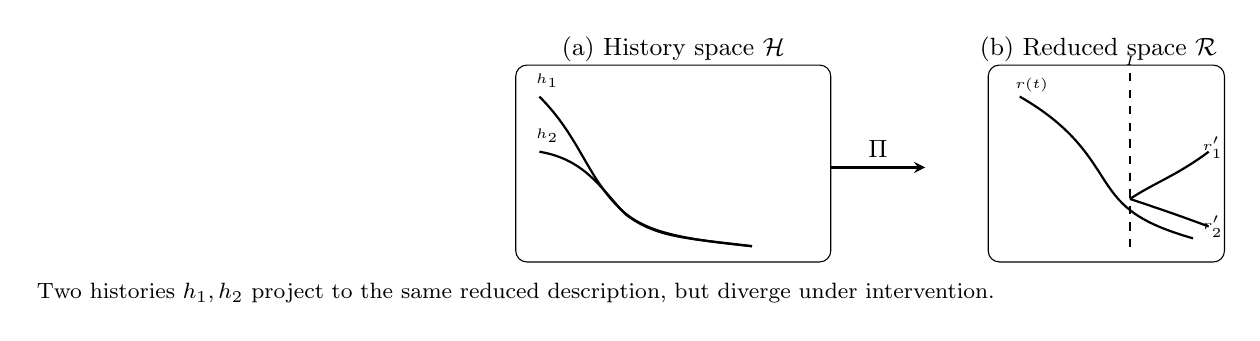
\begin{tikzpicture}[scale=1.0,>=stealth]
  % Left: history space
  \node[align=center] at (-4.0, 2.2) {\small (a) History space $\mathcal{H}$};
  \draw[rounded corners] (-6.0, -0.5) rectangle (-2.0, 2.0);

  \draw[thick] (-5.7, 1.6) .. controls (-5.2, 1.1) and (-5.1, 0.6) .. (-4.7, 0.2)
                       .. controls (-4.4, -0.1) and (-4.0, -0.2) .. (-3.0, -0.3);
  \draw[thick] (-5.7, 0.9) .. controls (-5.1, 0.8) and (-4.9, 0.4) .. (-4.6, 0.1)
                       .. controls (-4.2, -0.2) and (-3.8, -0.2) .. (-3.0, -0.3);

  \node[align=left] at (-5.6, 1.8) {\tiny $h_1$};
  \node[align=left] at (-5.6, 1.1) {\tiny $h_2$};

  % Projection arrow
  \draw[->,thick] (-2.0, 0.7) -- (-0.8, 0.7) node[midway,above] {\small $\Pi$};

  % Right: reduced space
  \node[align=center] at (1.4, 2.2) {\small (b) Reduced space $\mathcal{R}$};
  \draw[rounded corners] (0.0, -0.5) rectangle (3.0, 2.0);

  % merged reduced trajectory
  \draw[thick] (0.4, 1.6) .. controls (1.1, 1.2) and (1.3, 0.8) .. (1.5, 0.5)
                     .. controls (1.7, 0.2) and (1.9, 0.0) .. (2.6, -0.2);
  \node at (0.55,1.75) {\tiny $r(t)$};

  % intervention marker
  \draw[dashed] (1.8, 1.9) -- (1.8, -0.4);
  \node[align=center] at (1.8, 2.05) {\tiny $I$};

  % divergence under intervention (conceptual)
  \draw[thick] (1.8, 0.3) .. controls (2.1, 0.5) and (2.4, 0.6) .. (2.8, 0.9);
  \draw[thick] (1.8, 0.3) .. controls (2.1, 0.2) and (2.4, 0.1) .. (2.8, -0.05);

  \node[align=left] at (2.85, 0.95) {\tiny $r_1'$};
  \node[align=left] at (2.85, -0.05) {\tiny $r_2'$};

  % caption labels
  \node[align=left] at (-6.0, -0.9) {\footnotesize Two histories $h_1,h_2$ project to the same reduced description, but diverge under intervention.};
\end{tikzpicture}
\caption{The Unfaithful Cut (conceptual). Distinct admissible histories $h_1,h_2\in\mathcal{H}$
map under $\Pi$ to the same reduced description $r\in\mathcal{R}$, yet yield distinct outcomes
under the same intervention $I$, revealing a failure of counterfactual predictability in
$\Sigma_1$ descriptions and motivating the $\Sigma_2$ lift.}
\label{fig:unfaithful-cut}
\end{figure}